%!TEX root = UG_PhD_Defense.tex
\begin{frame}{\large Outline}
% Overview of the problems addressed and their solutions
\bi
	\item Problem Description and Motivation
	\item Preliminaries
	\item Unified Framework
	\bi
		\item Mathematical Challenges
	\ei
	\item Rectifiability Check
	\item Implementation
	\item Experimental Results
	\item Summary and Future work
	% \bi
	% 	\item Multi-error logic rectification
	% 	\item Approximate Computing
	% \ei 
	% \item Progress \& Objectives
	% \item Rectification of finite field arithmetic circuits
	% \bi
	% 	\item Problem Modeling over Finite Fields $\Fkk$
	% 	\item Single-fix rectification of Finite field arithmetic circuits
	% 	% \bi
	% 	% 	\item Application to circuit
	% 	% \ei
	% 	\item Multi-fix rectifiability of Finite field arithmetic circuits
	% 	\bi
	% 		\item Theory and Procedures
	% 		\item Application to circuit
	% 	\ei
	% \ei
\ei
\end{frame}


\begin{frame}{\large Problem Description: Rectification}

\begin{figure}[hbt]
\centering
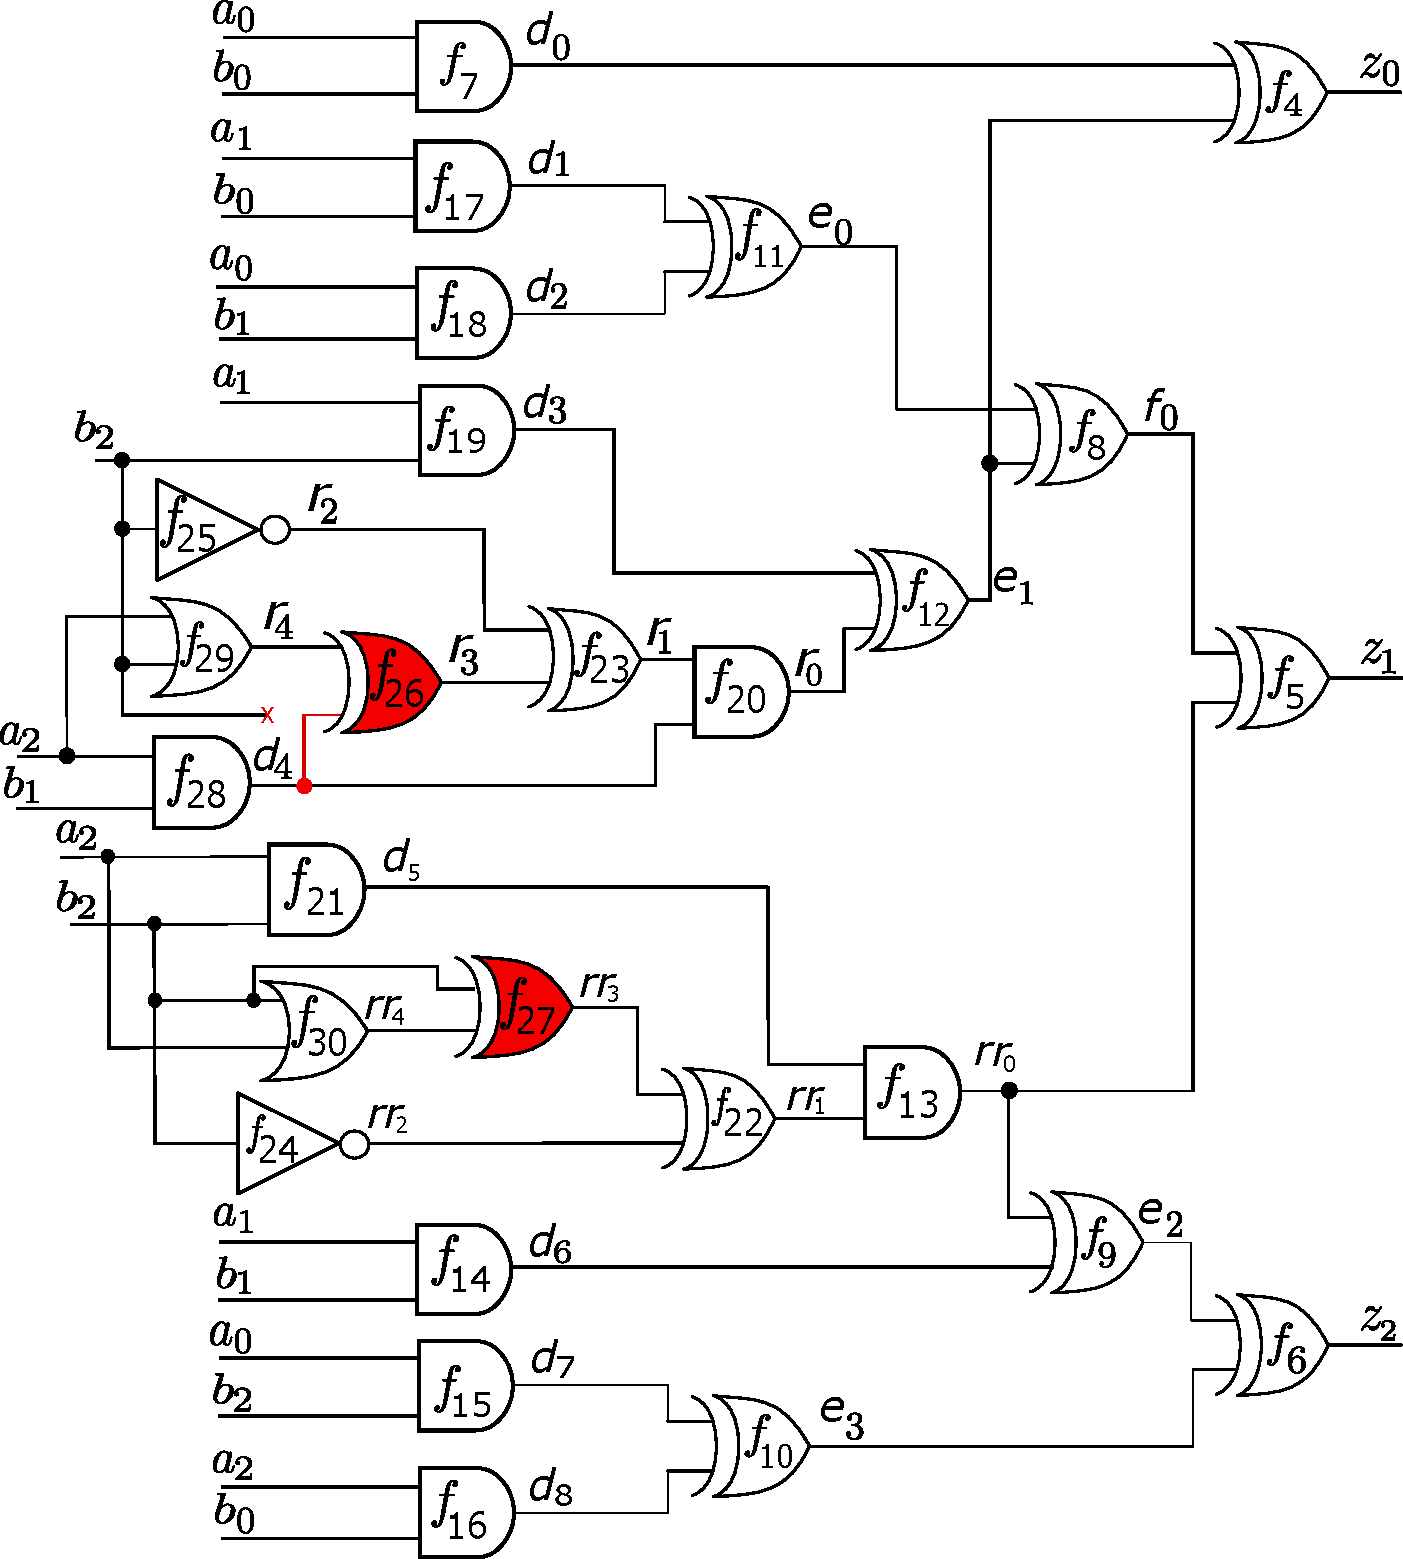
\includegraphics[scale=0.26]{mas_3_ddc_mfr_a.pdf}
\caption*{
% ($n$=3) with gate replacement bugs introduced at nets $d_5$ (AND replaced with an OR) and $d_2$ (AND replaced with an XOR), and a wire replacement bug at net $e_0$ (input shorted to $d_0$ instead of $d_1$).
}\label{fig:mas_bug_Wa}
\end{figure}
\end{frame}

\begin{frame}{\large Problem Description: Rectification}

\begin{figure}[hbt]
\centering
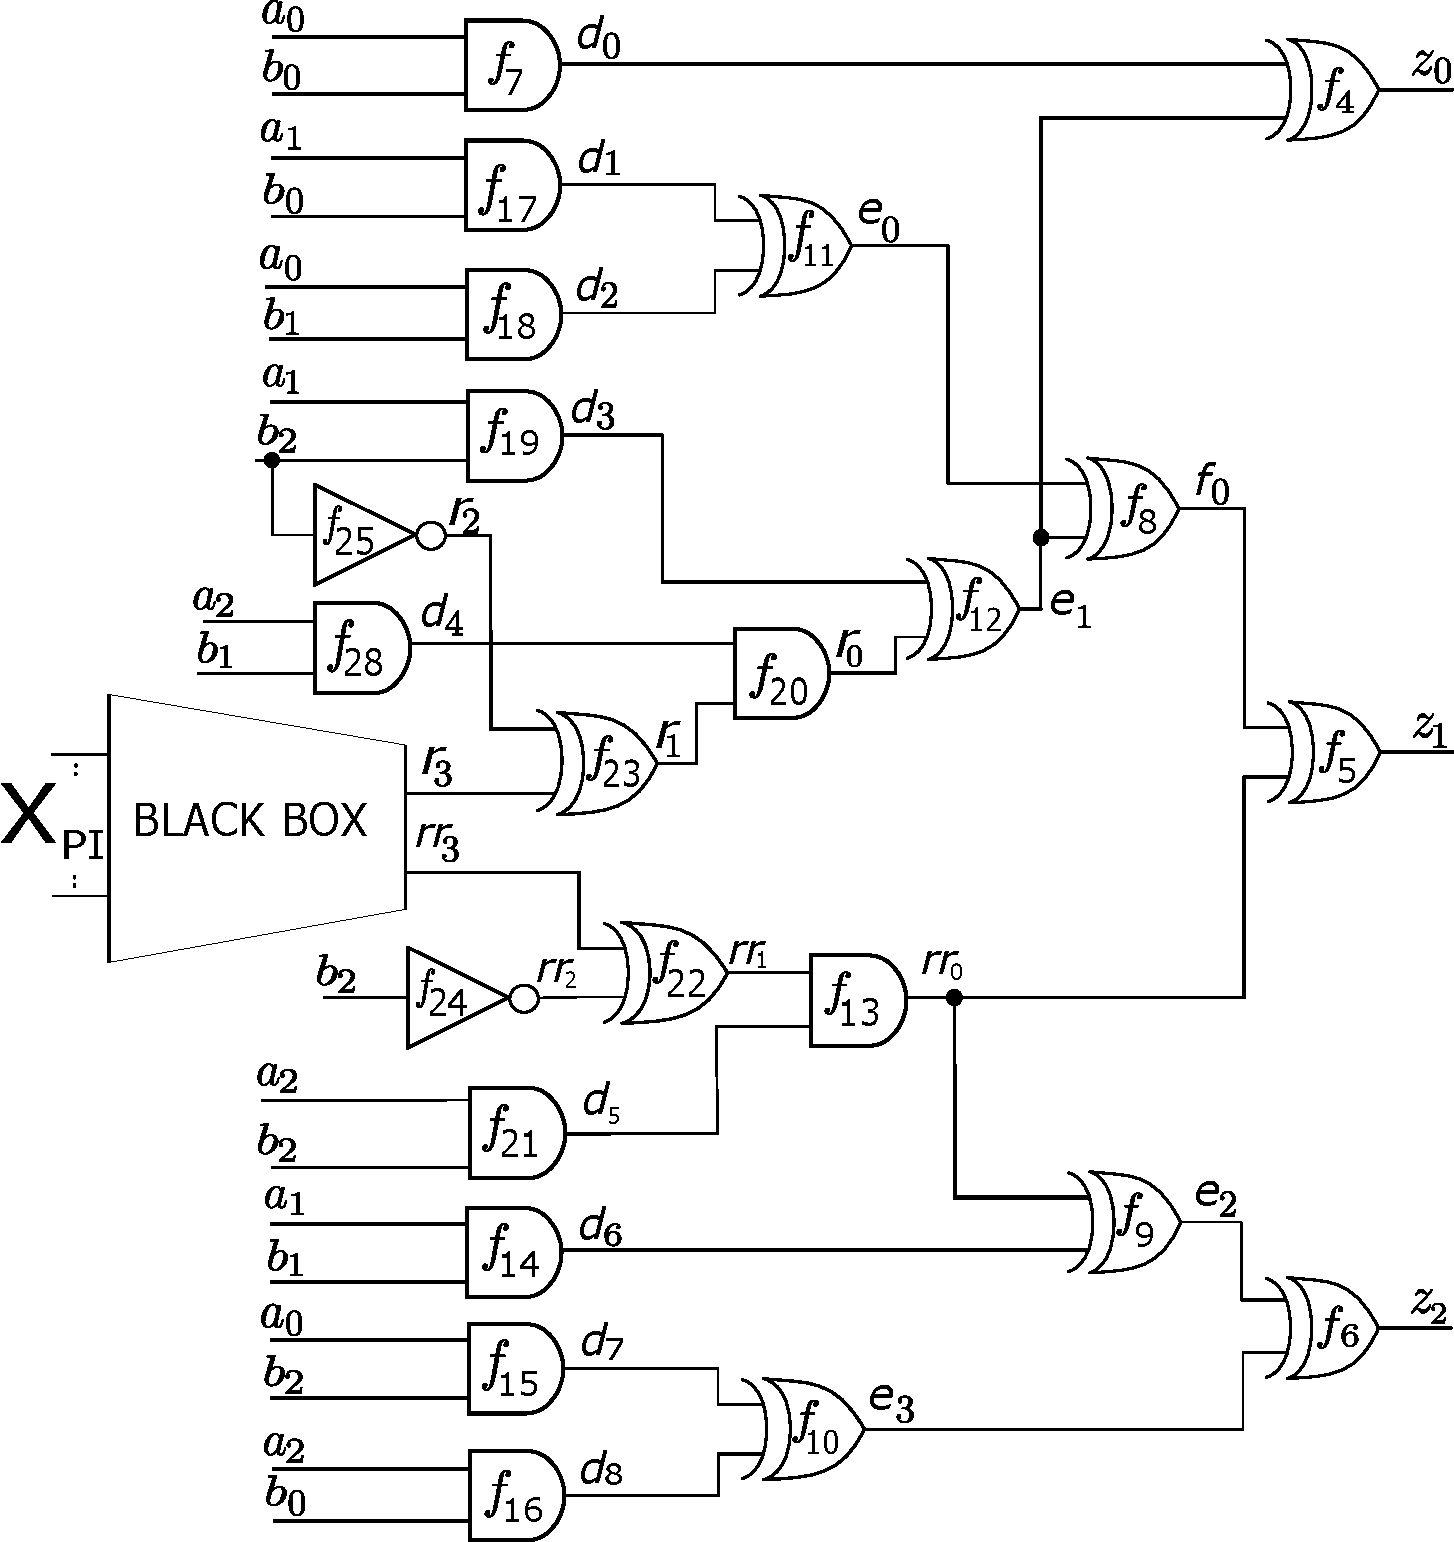
\includegraphics[scale=0.26]{mas_3_ddc_mfr_b_bb.pdf}
\caption*{
% ($n$=3) with gate replacement bugs introduced at nets $d_5$ (AND replaced with an OR) and $d_2$ (AND replaced with an XOR), and a wire replacement bug at net $e_0$ (input shorted to $d_0$ instead of $d_1$).
}\label{fig:mas_bug_Wb_bb}
\end{figure}
\end{frame}


\begin{frame}{\large Motivation: Finite Field Circuits}
\bi
	\item Applications:
	\bi
		\item Cryptography: RSA, Ellyptic Curve Cryptography (ECC) 
		\item Error Correcting Codes, Digital Signal Processing, RFID, etc.
		\pause
		\bi
			\item Crypto-system bugs can leak secret keys [{\it Biham. et al}, Crypto'08]
			\item RFID tag cloning could cause counterfeiting [{\it Batina. et al}, Security'09]
		\ei
		\pause
		\item Large datapath sizes ($n$) in ECC crypto systems 
		\bi
			\item $n=163, 233, 283, 409, 571$ (NIST standard)
		\ei
	\ei
	\pause
	\vspace{0.1in}
	\item Rectification Motivation: 
	\bi
		% \item Arithmetic circuits mostly custom designed; potential for errors
		\item Automated debugging
		\item Synthesize sub-functions as opposed to complete redesign
	\ei
\ei
\end{frame}
% \begin{frame}{\large Problem Description: Rectification}
% \bi 
% 	% \item Identify rectification target nets
% 	% \bi
% 	% 	\item Post-verification failure analysis
% 	% 	\item Primary output always a candidate for a correction
% 	% \ei
% 	\item Agnostic to the fault model, check for rectification at particular targets
% 	\bi
% 	\pause
% 		\item Single-fix Rectification (SFR)
% 		\bi
% 			\item Correct circuit by changing function at a single net
% 		\ei
% 	\ei
% 	\pause
% 	\vspace{0.1in}
% 	\vspace{0.1in}
% 	\vspace{0.1in}
% 	\item In a general setting, SFR might not be desired or may not exist
% 	\bi
% 	\pause
% 	\item Multi-fix Rectification (MFR)
% 	\bi
% 		\item Correct circuit by changing functions at multiple nets
% 		\item Contribution: Multi-fix rectifiability setup and check
% 	\ei
% 	\ei
% \ei
% \end{frame}

%https://ieeexplore.ieee.org/document/8405614 - cryptography

% \begin{frame}{\large Motivation: Approximate Computing}

% \bi
% 	\item Trade off accuracy for cost savings [{\it Kulkarni. et al}, VLSI'11]
% 	\item Synthesize approximate circuit by performing ECO style patch on original exact circuit
% \ei
% %\item Application to approximate circuits
% % \bi
% % 	\item Exact efficient implementation given
% % 	\item Rectify it minimally to match a new approximate $spec$
% % \ei
% \begin{figure}[hbt]
% \centering
% 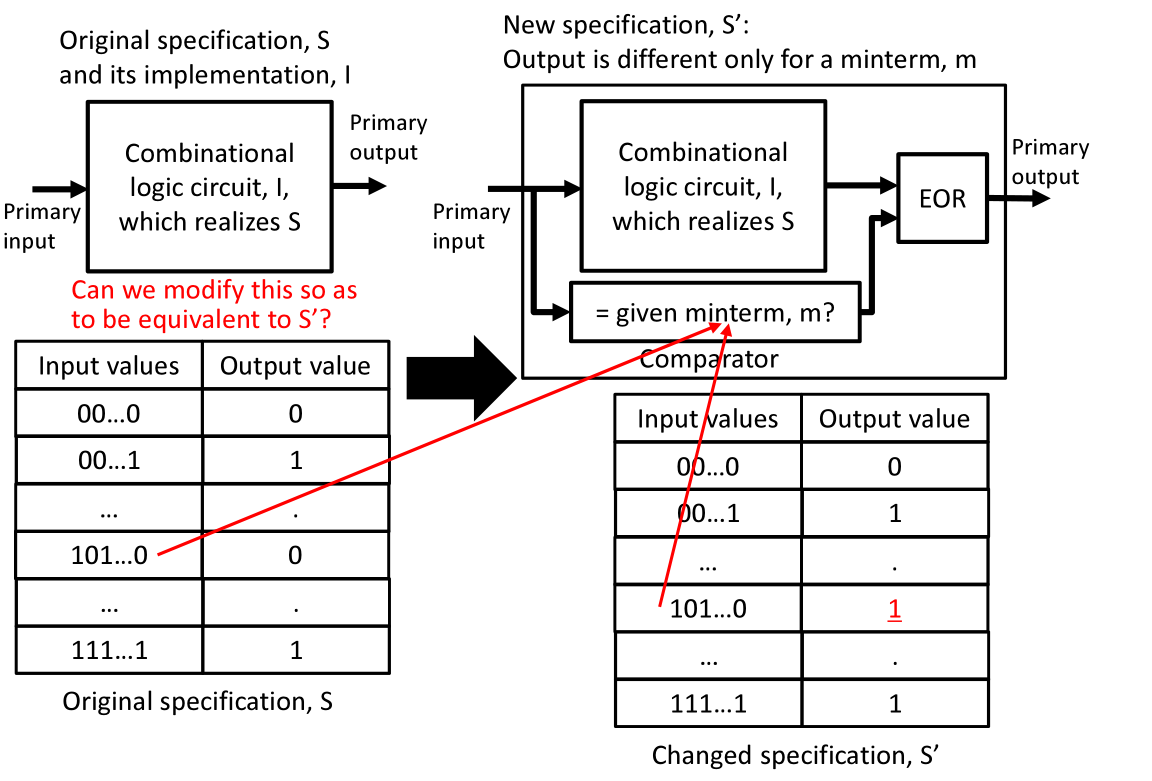
\includegraphics[scale = 0.25]{minterm.png}
%     \caption{Single minterm functional change. EOR = Ex-OR gate}
%     \label{fig:mint}
% \end{figure}
% \end{frame}

% \begin{frame}{\large Focus: Integer Arithmetic Circuits}
% \bi
% 	\item Approximate integer primitives
% 	\bi
% 		\item Exploits error resilience of real-world applications
% 		\item Neuromorphic Architectures, Data mining, Machine Learning, etc.
% 		\item Quantification:
% 		\bi
% 			\item Magnitude: Maximum deviation of the approximate output as
% compared to the defined constraint
% 			\item Frequency: Ratio of the number of magnitude deviations from the correct
% value to the total number of outputs
% 		\ei
% 	\ei
% 	\vspace{0.1in}
% 	\item {\it Lamb} investigated SFR of approximate integer multipliers
% 	\bi
% 		\item Single cube error (frequency) introduced across two output bits (magnitude)
% 		% \bi
% 		% 	\item Translates to corruption of a single minterm entry in the original truth table for respective outputs
% 		% \ei
% 		% \item Observations from experiments on 2/3/4-bit multiplier circuits
% 		\bi
% 			\item {\red 4\%} of 2-bit, {\red 1.6\%} of 3-bit approximate specs admits SFR
% 			\item 4-bit circuit has {\red zero} SFR points
% 		\ei
% 	\ei
% \ei
% \end{frame}



% \begin{frame}{\large Previous Approaches: Verification}
% \bi
% 	\item Canonical Decision Diagrams
% 	\bi
% 		\item BDDs, BMDs, and their variants
% 		\item Infeasible for arithmetic circuits
% 	\ei
% 	\vspace{0.1in}
% 	\item Combinational Equivalence Checking using SAT
% 	\bi
% 		\item AIG + SAT: Work for structurally similar circuits
% 	\ei
% 	\vspace{0.1in}
% 	\item Verification using computer algebra
% 	\bi
% 		\item Formulations in $\Zkk$: [Namrata et al, TCAD'07]
% 		\item Formulations in $\Fkk$: [Lv et al, TCAD’13] [Pruss et al, TCAD'16]
% 		\item Formulations in $\F_2$: [Cunxi et al, ASP-DAC'17]
% 		\item Integer arithmetic circuits: [Ciesielski et al, DAC'15] [A.Sayed et al, DATE’16] [D. Ritirc et al, FMCAD’17]
% 		[A. Sayed et al, FMCAD'16]
% 	\ei
% \ei
% \end{frame}

% \begin{frame}{\large Previous Approaches: Rectification}
% % Ideas came from ATPG, Boolean Differences, 
% % Based on Boolean reasoning engines
% % Then SAT solvers became efficient and replaced those
% % SAT based decision procedure for rectification test 
% % if it passes, the way the problem is set-up Craig interpolants
% % can be used to compute the rf
% % 12 bit: then we started looking into this problem. Our group has
% % already done on verification using computer algebra which is
% % scalable on FF ckts, from there we started looking into rectification using this formulation